% Synchronized to r35303

\marklabel{sec:OPTSAMBAPOINTANDPRINT:XP}{\section{SAMBA\_LPD - Point'n'Print Configuration using Windows XP}}

This section describes how the Point'n'Print functionality is configured
using a Windows XP client.

First, the print server must be ``found''. This can i.e. be accomplished
using the networking environment.
(Fig.~\ref{fig:sambalpd:icon-networking-environment} to
\ref{fig:sambalpd:networking-environment:4}). In the current example the
Workgroup is called ``GARDEN'' and the fli4l server ``ODIN''. The printer
for which a driver should be installed is a Brother HL-2240D.

\begin{figure}[hbt!]
\centering

\includegraphics[]{image001}
\caption{Networking Environment: Desktop Symbol}
\label{fig:sambalpd:icon-networking-environment}
\end{figure}

\begin{figure}[hbt!]
\centering
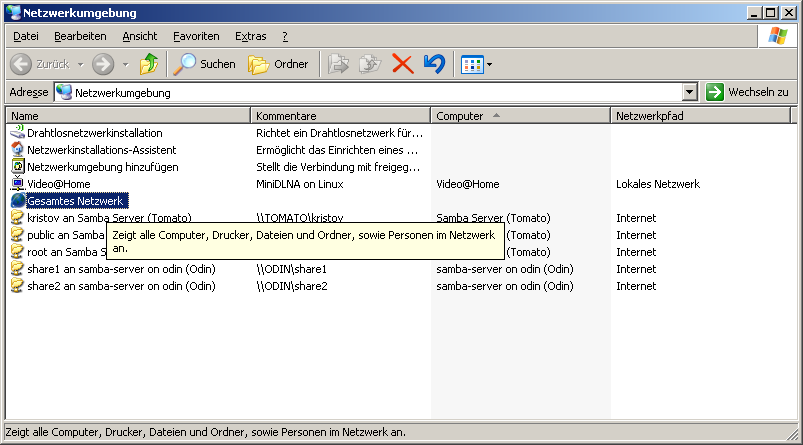
\includegraphics[width=\columnwidth]{image002}
\caption{Networking Environment: Common View}
\label{fig:sambalpd:networking-environment:1}
\end{figure}

\begin{figure}[hbt!]
\centering
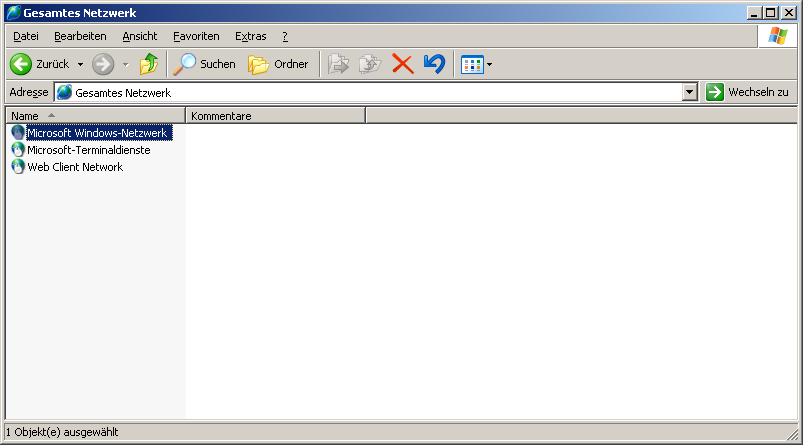
\includegraphics[width=\columnwidth]{image003}
\caption{Networking Environment: Select the Network Type}
\label{fig:sambalpd:networking-environment:2}
\end{figure}

\begin{figure}[hbt!]
\centering
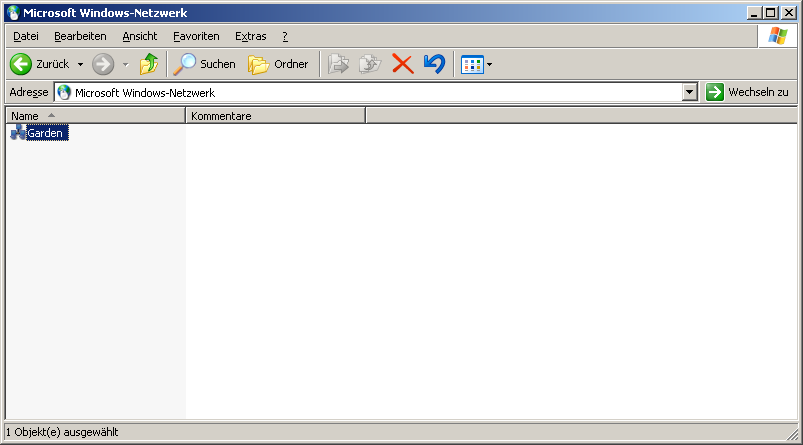
\includegraphics[width=\columnwidth]{image004}
\caption{Networking Environment: Select the Workgroup}
\label{fig:sambalpd:networking-environment:3}
\end{figure}

\begin{figure}[hbt!]
\centering
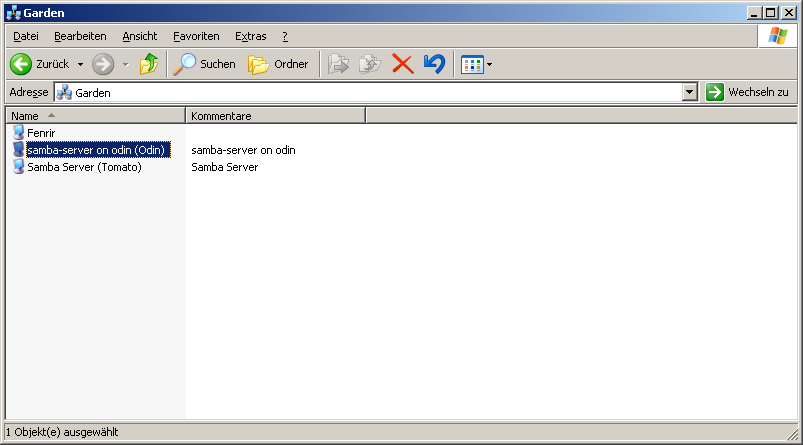
\includegraphics[width=\columnwidth]{image005}
\caption{Networking Environment: Select the fli4l print server}
\label{fig:sambalpd:networking-environment:4}
\end{figure}

When the fli4l print server is found, open a window that displays the services
offered by double-clicking its icon.
(Fig.~\ref{fig:sambalpd:services}). Select ``Printer and Fax Devices''. The
following list shows all printers shared by the fli4l server. Select the desired
printer now and display its context menu entry ``Properties''
(Fig.~\ref{fig:sambalpd:printerproperties}). You will get a message
(Fig.~\ref{fig:sambalpd:no-driver:1}) stating that there is no driver installed
for this printer (which is true). Cancel this message with ``No'' because the
driver will get installed using another method.

\begin{figure}[hbt!]
\centering
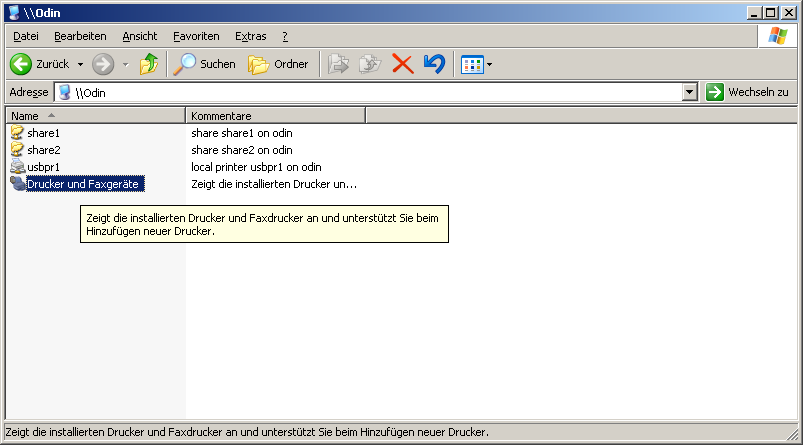
\includegraphics[width=\columnwidth]{image006}
\caption{Server Services}
\label{fig:sambalpd:services}
\end{figure}

\begin{figure}[hbt!]
\centering
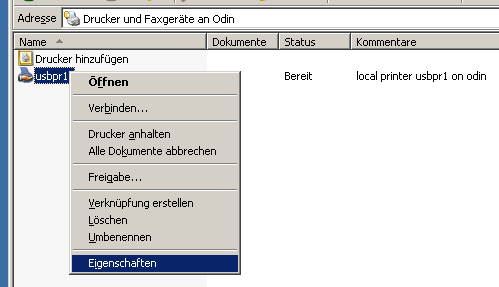
\includegraphics[width=\columnwidth]{image007}
\caption{Selection of printer properties}
\label{fig:sambalpd:printerproperties}
\end{figure}

\begin{figure}[hbt!]
\centering
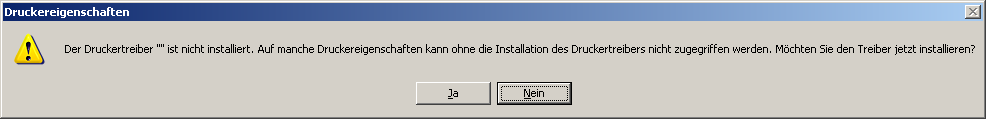
\includegraphics[width=\columnwidth]{image008}
\caption{Printer driver missing (1)}
\label{fig:sambalpd:no-driver:1}
\end{figure}

This will open the properties dialog. There you have to select the tab
``Advanced'' and then the button ``New Driver''
(Fig.~\ref{fig:sambalpd:props-start-setup}). This leads to the start of the
``Printer installation wizard''
(Fig.~\ref{fig:sambalpd:setup-start}). With ``Next'' proceed to the
driver selection (Fig.~\ref{fig:sambalpd:setup-choose-driver:1}). If the
desired driver is not found, select a path to a driver directory
via ``Volume'' (i.e. a directory on the printer's installation CD)
in this case a second list of drivers available there will be shown
to choose a driver from (Fig.~\ref{fig:sambalpd:setup-choose-driver:2}).
After confirming the selection by clicking ``Next '' a message will be
displayed that the wizard has completed successfully.
(Fig.~\ref{fig:sambalpd:setup-end}). However, this is not true because
only after selecting the ``Finish'' the driver will be copied to the
fli4l server and then activated there
(Fig.~\ref{fig:sambalpd:driver-copy}).

\begin{figure}[hbt!]
\centering
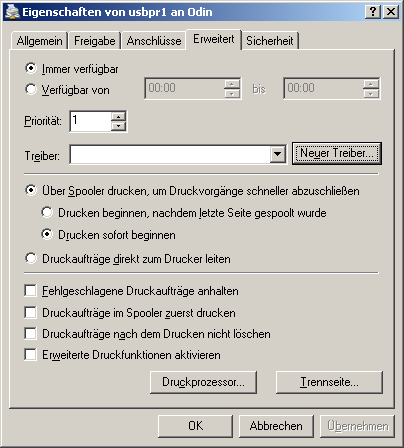
\includegraphics[width=0.8\columnwidth]{image009}
\caption{Printer properties: Start of driver installation}
\label{fig:sambalpd:props-start-setup}
\end{figure}

\begin{figure}[hbt!]
\centering
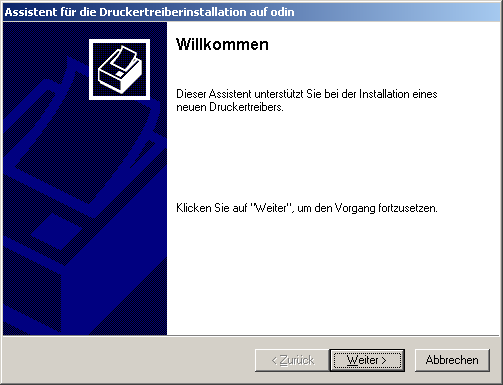
\includegraphics[width=\columnwidth]{image010}
\caption{Printer properties}
\label{fig:sambalpd:setup-start}
\end{figure}

\begin{figure}[hbt!]
\centering
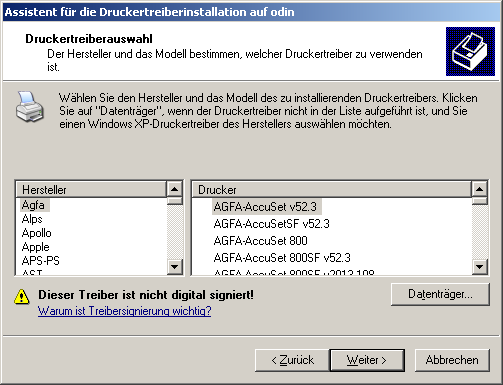
\includegraphics[width=0.7\columnwidth]{image011}
\caption{Driver installation: Driver selection 1}
\label{fig:sambalpd:setup-choose-driver:1}
\end{figure}

\begin{figure}[hbt!]
\centering
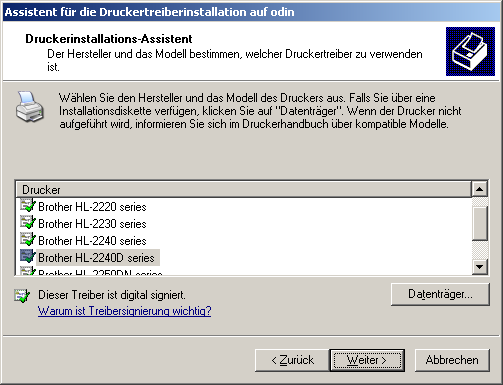
\includegraphics[width=0.7\columnwidth]{image012}
\caption{Driver installation: Driver selection 2}
\label{fig:sambalpd:setup-choose-driver:2}
\end{figure}

\begin{figure}[hbt!]
\centering
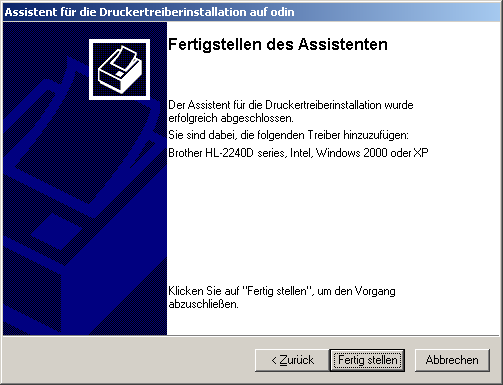
\includegraphics[width=\columnwidth]{image013}
\caption{Driver installation: Completing the wizard}
\label{fig:sambalpd:setup-end}
\end{figure}

\begin{figure}[hbt!]
\centering
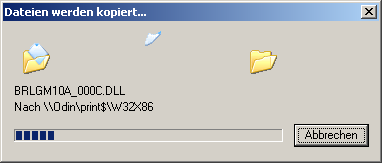
\includegraphics[width=\columnwidth]{image014}
\caption{Driver installation: Copying the driver}
\label{fig:sambalpd:driver-copy}
\end{figure}

Then you see in the properties dialog that the previously selected and
installed driver is noted under ``Drivers''
(Fig.~\ref{fig:sambalpd:setup-completed}). Now the Properties dialog must
be terminated via ``OK''. Here again you get a message that the
driver is missing (Fig.~\ref{fig:sambalpd:no-driver:2}), which is nonsense
this time because the driver is now installed. Therefore select ``No'' here
again to confirm that you really don't want to install a driver now.
Now go back to the ``Printer and Fax devices'', Windows has renamed the
printer according to the selected driver (Fig.~\ref{fig:sambalpd:installed}).
This is not a problem, accessing the fli4l printer server is still possible.

\begin{figure}[hbt!]
\centering
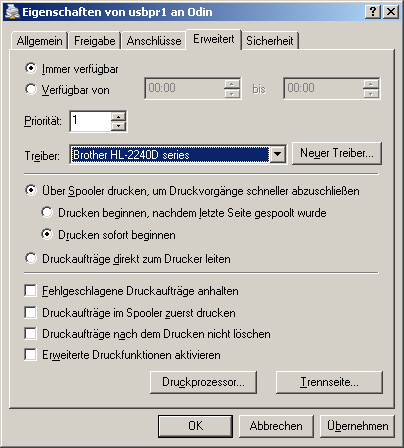
\includegraphics[width=\columnwidth]{image015}
\caption{Driver installation completed}
\label{fig:sambalpd:setup-completed}
\end{figure}

\begin{figure}[hbt!]
\centering
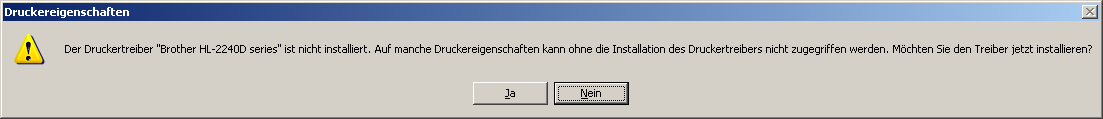
\includegraphics[width=\columnwidth]{image016}
\caption{Printer driver missing(2)}
\label{fig:sambalpd:no-driver:2}
\end{figure}

\begin{figure}[hbt!]
\centering
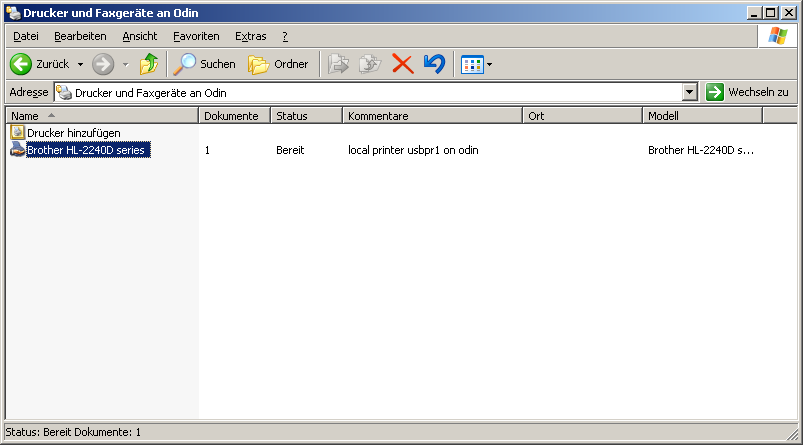
\includegraphics[width=0.8\columnwidth]{image017}
\caption{Part 1 of the printer installation completed}
\label{fig:sambalpd:installed}
\end{figure}

However, we are not done yet. The printer's default settings have to be set once.
Go back to the printer properties dialog (Fig.~\ref{fig:sambalpd:printerproperties})
and select the button ``Default settings'' in the tab ``Advanced''.
(Fig.~\ref{fig:sambalpd:props-reloaded:1}). (This button was previously
not displayed there, so we could not do this earlier).
Now a driver-dependent dialog is opened
(Fig.~\ref{fig:sambalpd:props-reloaded:2}). Specify the desired printer
settings in this dialog. As a rule of thumb it is necessary to set the
paper size from ``Letter'' to ``A4''. If all settings seem to be correct,
it is nevertheless necessary to change a setting and restore it
again ~-- this is necessary for Windows to really store the settings
on the fli4l server on exiting the dialog via ``OK''.

\begin{figure}[hbt!]
\centering
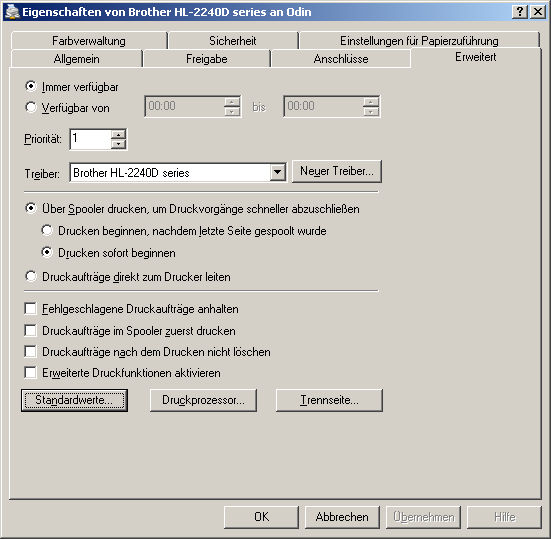
\includegraphics[width=0.8\columnwidth]{image018}
\caption{Set the default values (1)}
\label{fig:sambalpd:props-reloaded:1}
\end{figure}

\begin{figure}[hbt!]
\centering
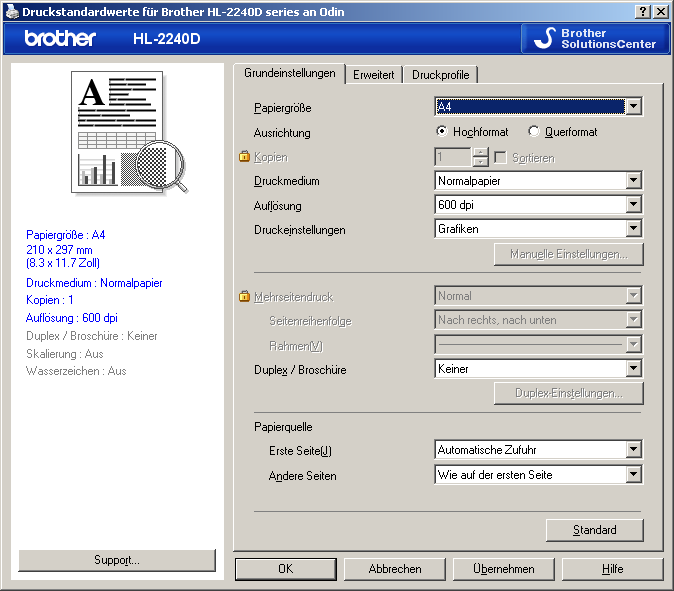
\includegraphics[width=\columnwidth]{image019}
\caption{Set the default values (2)}
\label{fig:sambalpd:props-reloaded:2}
\end{figure}

Now we really reached the end! The server-side configuration is complete.
If you want to use the printer you just set up, you have to connect to it
(Fig.~\ref{fig:sambalpd:connect:1}). The warning message that appears abaout
the dangers of driver installation (Fig.~\ref{fig:sambalpd:connect:2}) must be
confirmed. Then the printer connected appears in the printer environment
(Fig.~\ref{fig:sambalpd:printer-environment}). Here we go!

\begin{figure}[hbt!]
\centering
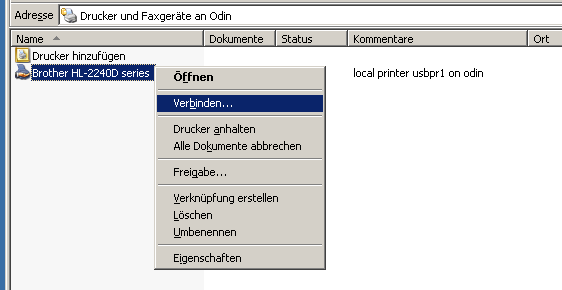
\includegraphics[width=\columnwidth]{image020}
\caption{Connect to the printer (1)}
\label{fig:sambalpd:connect:1}
\end{figure}

\begin{figure}[hbt!]
\centering
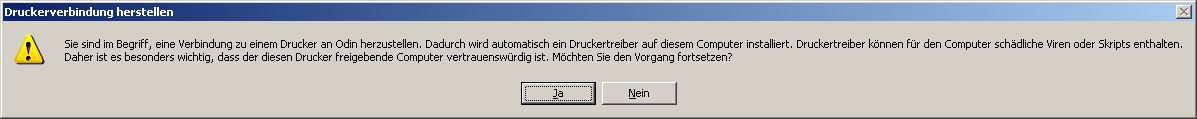
\includegraphics[width=\columnwidth]{image021}
\caption{Connect to the printer (2)}
\label{fig:sambalpd:connect:2}
\end{figure}

\begin{figure}[hbt!]
\centering
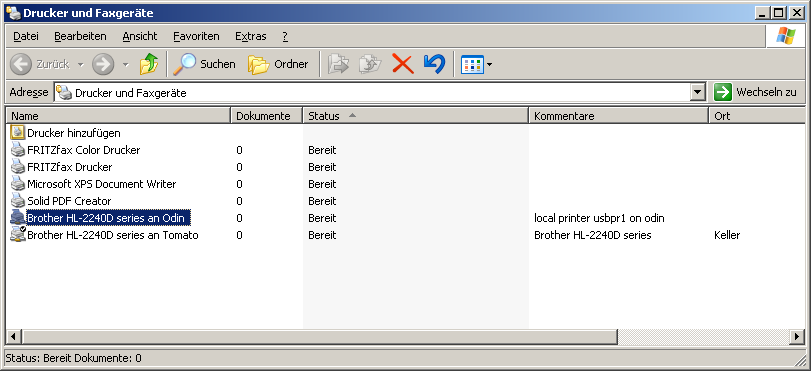
\includegraphics[width=\columnwidth]{image022}
\caption{Connected Printer in Printer Environment}
\label{fig:sambalpd:printer-environment}
\end{figure}
